% Source: Weinberg GR, physical PDF p. 306 (printed p. 284).
% Coverage: Figure 10.1, Weber detector intensity versus sidereal time.
% Status: source plot extracted at high resolution; source-reviewed and
%         compile-clean.
% Uncertainties: none.

\begingroup
\renewcommand{\thefigure}{10.1}
\begin{figure}[t]
\centering
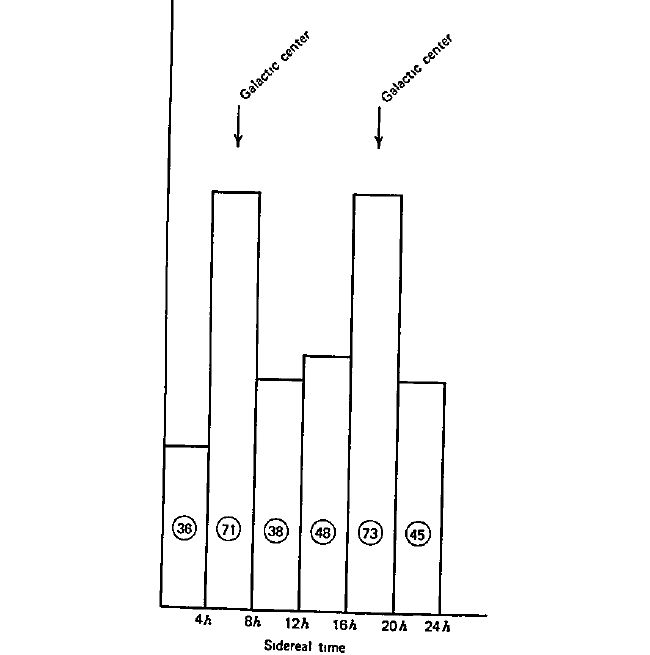
\includegraphics[width=0.76\textwidth]{figures/chapter10/fig10-01.png}
\caption{Evidence for gravitational radiation emanating from the center of
the galaxy.\hyperref[ch10-ref-18]{\textsuperscript{18}} The detector
intensity observed by Weber is plotted here (in arbitrary units) against
sidereal time. Arrows mark the sidereal times at which the antenna is most
nearly perpendicular to the line of sight to the center of the galaxy.
Numbers in circles are the observed numbers of coincidences in each time
interval.}
\label{fig:10.1}
\end{figure}
\endgroup
